\documentclass{article}

\usepackage{graphicx}
\usepackage{tikz}
\usepackage{tikzsymbols}
\usetikzlibrary{calc,patterns,shapes.geometric}
\pagestyle{empty}
\usepackage[margin=0pt]{geometry}
\geometry{papersize={14in,12in}}

\def\centerarc[#1](#2)(#3:#4:#5){\draw[#1] ($(#2)+({#5*cos(#3)},{#5*sin(#3)})$) arc (#3:#4:#5);}

\begin{document}
	\begin{figure}
		\centering
		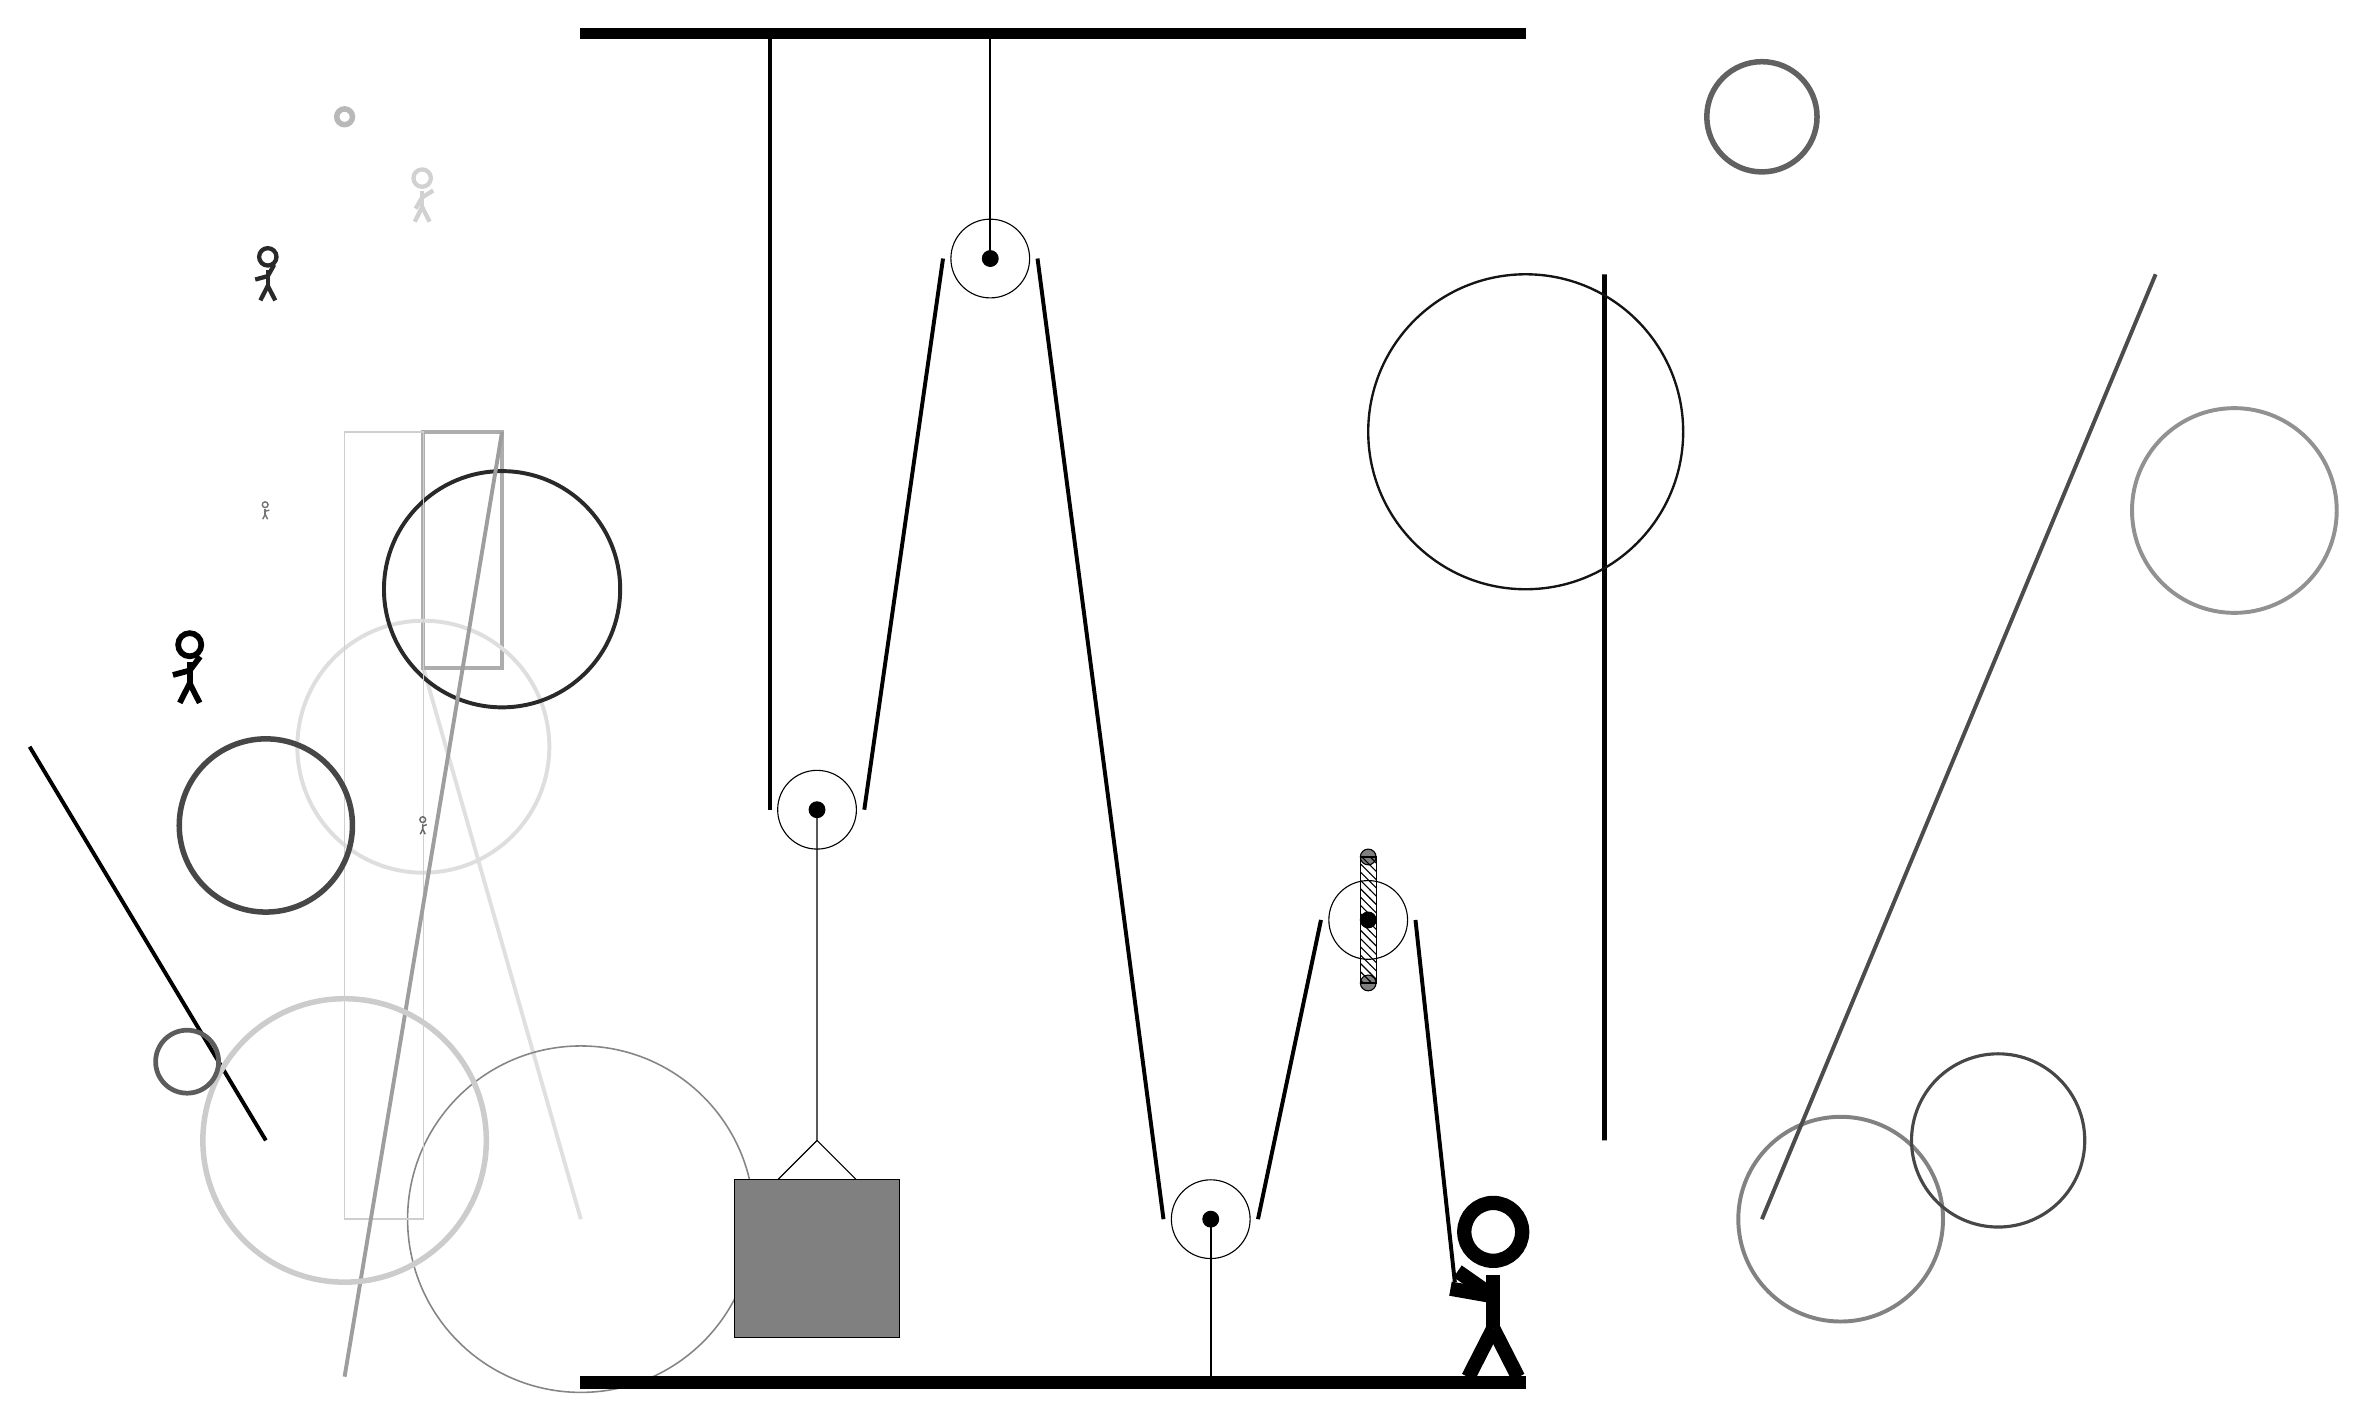
\begin{tikzpicture}
			%%%%% START %%%%%
			
			\draw[fill=black] (-2, 14) rectangle (10, 14.125);
			
			\draw (1, 4.2) circle (0.5);
			\draw[fill=black] (1, 4.2) circle (0.1);
			
			\draw (3.2, 11.2) circle (0.5);
			\draw[fill=black] (3.2, 11.2) circle (0.1);
			\draw[thick] (3.2, 11.2) -- (3.2, 14);
			
			\draw (6, -1) circle (0.5);
			\draw[fill=black] (6, -1) circle (0.1);
			\draw[thick] (6, -1) -- (6, -3);
			
			\draw[line width=0.5mm, color=black!12](-2, -1) -- (-4, 6);
			
			\draw [line width=0.5mm, color=black!49](14, -1) circle (1.3);
			\draw [line width=0.4mm, color=black!72](16, 0) circle (1.1);
			\draw[line width=0.5mm, color=black!32] (-4, 6) rectangle (-3, 9);
			\draw [line width=0.5mm, color=black!13](-4, 5) circle (1.6);
			\draw [line width=0.7mm, color=black!62](13, 13) circle (0.7);
			\node[line width=0.5mm, color=black!100] at (-7, 6) {\Strichmaxerl[4][15][53]};
			\node[line width=0.3mm, color=black!84] at (-6, 11) {\Strichmaxerl[3][15][61]};
			\draw [line width=0.2mm, color=black!48](-2, -1) circle (2.2);
			
			\draw [line width=0.5mm, color=black!84](-3, 7) circle (1.5);
			
			\draw[line width=0.2mm, color=black!19] (-4, -1) rectangle (-5, 9);
			
			\draw [line width=0.7mm, color=black!28](-5, 13) circle (0.1);
			\draw[line width=0.5mm, color=black!38](-5, -3) -- (-3, 9);
			
			\draw[line width=0.6mm, color=black!99] (11, 0) rectangle (11, 11);
			\draw [line width=0.3mm, color=black!92](10, 9) circle (2.0);
			\draw[line width=0.5mm, color=black!100](-6, 0) -- (-9, 5);
			\draw[line width=0.5mm, color=black!70](13, -1) -- (18, 11);
			
			\draw [line width=0.7mm, color=black!20](-5, 0) circle (1.8);
			\node[line width=0.2mm, color=black!18] at (-4, 12) {\Strichmaxerl[3][60][32]};
			\node[line width=0.5mm, color=black!59] at (-4, 4) {\Strichmaxerl[1][88][21]};
			\node[line width=0.5mm, color=black!54] at (-6, 8) {\Strichmaxerl[1][90][12]};
			
			\draw [line width=0.6mm, color=black!64](-7, 1) circle (0.4);
			\draw [line width=0.7mm, color=black!72](-6, 4) circle (1.1);
			\draw [line width=0.5mm, color=black!43](19, 8) circle (1.3);
			
			\draw[fill=white](8, 2.8) circle (0.5);
			\draw[fill=black] (8, 2.8) circle (0.1);
			\draw[fill=black!50] (8, 3.6) circle (0.1);
			\draw[fill=black!50] (8, 2.0) circle (0.1);
			\draw[pattern=north west lines, pattern color=black] (7.9, 3.6) rectangle (8.1, 2.0);
			
			\draw (1, 4.2) -- (1, 0) -- (0.5, -0.5);
			\draw (1, 0) -- (1.5, -0.5);
			\draw[fill=black!50] (-0.05, -0.5) rectangle (2.05, -2.5);
			
			\draw[line width=0.5mm] (0.4, 14) -- (0.4, 4.2);
			\centerarc[line width=0.5mm](1, 4.2)(180:360:0.6);
			\draw[line width=0.5mm](1.6, 4.2) -- (2.6, 11.2);
			\centerarc[line width=0.5mm](3.2, 11.2)(0:180:0.6);
			\draw[line width=0.5mm](3.8, 11.2) -- (5.4, -1);
			\centerarc[line width=0.5mm](6, -1)(180:360:0.6);
			\draw[line width=0.5mm](6.6, -1) -- (7.4, 2.8);
			\centerarc[line width=0.5mm](8, 2.8)(0:180:0.6);
			\draw[line width=0.5mm](8.6, 2.8) -- (9.1, -1.8);
			
			\node at (9.5, -1.9) {\Strichmaxerl[10][-35][170]};
			
			\draw[fill=black] (-2, -3) rectangle (10, -3.15);
			
			%%%%% END %%%%%
		\end{tikzpicture}
	\end{figure}	
\end{document}